\begin{figure}
%	 pgfplots style "layerwiseexperimentdefault"
	  \pgfkeys{/pgfplots/layerwiseexperimentdefault/.style={
	      width=\linewidth,
	      height=0.13\textheight,
	      every axis plot/.append style={line width = 1.2pt},
	      tick pos = left,
	      xmajorticks = true,
	      ymajorticks = true,
	      ylabel near ticks,
	      xlabel near ticks,
	      xtick align = inside,
	      ytick align = inside,
	      ytick={-1,0,1},
	      legend cell align = left,
	      legend columns = 1,
	      legend pos = south east,
	      legend style = {
	        fill opacity = 0.9,
	        text opacity = 1,
	        font = \small,
	      },
	      xticklabel style = {font = \small, inner xsep = -5ex},
	      xlabel style = {font = \small},
	      axis line style = {black},
	      yticklabel style = {font = \small, inner ysep = -4ex},
	      ylabel style = {font = \small},
	      title style = {font = \small, inner ysep = -3ex},
	      grid = major,
	      grid style = {dashed}
	    }
	  }
	
	\centering
	\begin{subfigure}[t]{0.4\textwidth}
%		 customize "zmystyle" as you wish
		\pgfkeys{/pgfplots/zmystyle/.style={layerwiseexperimentdefault,
		   title = {Network}, ylabel=Gradient\\Element, ylabel style={align=left}, xticklabels = {}
		 }}
		% This file was created by tikzplotlib v0.9.8.
\begin{tikzpicture}

\definecolor{color0}{rgb}{0.12156862745098,0.466666666666667,0.705882352941177}

\begin{axis}[
axis line style={white},
log basis x={10},
tick align=outside,
xmajorticks=false,
xmin=0.9, xmax=233063278.37446,
xmode=log,
xtick style={color=white!15!black},
ymajorticks=false,
ymin=-1.1000000834465, ymax=1.1000000834465,
zmystyle
]
\draw[draw=white,fill=color0,line width=0.02pt] (axis cs:0.9,-1.1000000834465) rectangle (axis cs:0.9,-0.990000069141388);
\draw[draw=white,fill=color0,line width=0.02pt] (axis cs:0.9,-0.990000009536743) rectangle (axis cs:0.9,-0.879999995231628);
\draw[draw=white,fill=color0,line width=0.02pt] (axis cs:0.9,-0.880000054836273) rectangle (axis cs:0.9,-0.770000040531158);
\draw[draw=white,fill=color0,line width=0.02pt] (axis cs:0.9,-0.770000040531158) rectangle (axis cs:0.9,-0.660000026226044);
\draw[draw=white,fill=color0,line width=0.02pt] (axis cs:0.9,-0.660000026226044) rectangle (axis cs:0.9,-0.550000011920929);
\draw[draw=white,fill=color0,line width=0.02pt] (axis cs:0.9,-0.550000011920929) rectangle (axis cs:0.9,-0.439999997615814);
\draw[draw=white,fill=color0,line width=0.02pt] (axis cs:0.9,-0.440000057220459) rectangle (axis cs:23.9,-0.330000042915344);
\draw[draw=white,fill=color0,line width=0.02pt] (axis cs:0.9,-0.330000042915344) rectangle (axis cs:868.9,-0.220000028610229);
\draw[draw=white,fill=color0,line width=0.02pt] (axis cs:0.9,-0.220000028610229) rectangle (axis cs:38909.9,-0.110000014305115);
\draw[draw=white,fill=color0,line width=0.02pt] (axis cs:0.9,-0.110000006854534) rectangle (axis cs:92649650.9,7.45058059692383e-09);
\draw[draw=white,fill=color0,line width=0.02pt] (axis cs:0.9,2.23517417907715e-08) rectangle (axis cs:21858861.9,0.110000036656857);
\draw[draw=white,fill=color0,line width=0.02pt] (axis cs:0.9,0.110000014305115) rectangle (axis cs:35123.9,0.220000028610229);
\draw[draw=white,fill=color0,line width=0.02pt] (axis cs:0.9,0.220000028610229) rectangle (axis cs:2220.9,0.330000042915344);
\draw[draw=white,fill=color0,line width=0.02pt] (axis cs:0.9,0.330000042915344) rectangle (axis cs:686.9,0.440000057220459);
\draw[draw=white,fill=color0,line width=0.02pt] (axis cs:0.9,0.439999997615814) rectangle (axis cs:276.9,0.550000011920929);
\draw[draw=white,fill=color0,line width=0.02pt] (axis cs:0.9,0.550000011920929) rectangle (axis cs:95.9,0.660000026226044);
\draw[draw=white,fill=color0,line width=0.02pt] (axis cs:0.9,0.660000026226044) rectangle (axis cs:27.9,0.770000040531158);
\draw[draw=white,fill=color0,line width=0.02pt] (axis cs:0.9,0.770000040531158) rectangle (axis cs:25.9,0.880000054836273);
\draw[draw=white,fill=color0,line width=0.02pt] (axis cs:0.9,0.879999995231628) rectangle (axis cs:117.9,0.990000009536743);
\draw[draw=white,fill=color0,line width=0.02pt] (axis cs:0.9,0.990000069141388) rectangle (axis cs:0.9,1.1000000834465);
\end{axis}

\end{tikzpicture}

		
		\vspace{-0.1cm}
%		customize "zmystyle" as you wish
		\pgfkeys{/pgfplots/zmystyle/.style={layerwiseexperimentdefault,
		   ylabel=Gradient\\Element, ylabel style={align=left}
		 }}
		% This file was created by tikzplotlib v0.9.8.
\begin{tikzpicture}

\definecolor{color0}{rgb}{1,0.498039215686275,0.0549019607843137}

\begin{axis}[
axis line style={white},
log basis x={10},
tick align=outside,
xmajorticks=false,
xmin=0.9, xmax=141796339.435146,
xmode=log,
xtick style={color=white!15!black},
ymajorticks=false,
ymin=-1.1000000834465, ymax=1.1000000834465,
zmystyle
]
\draw[draw=white,fill=color0,line width=0.02pt] (axis cs:0.9,-1.1000000834465) rectangle (axis cs:0.9,-0.990000069141388);
\draw[draw=white,fill=color0,line width=0.02pt] (axis cs:0.9,-0.990000009536743) rectangle (axis cs:0.9,-0.879999995231628);
\draw[draw=white,fill=color0,line width=0.02pt] (axis cs:0.9,-0.880000054836273) rectangle (axis cs:0.9,-0.770000040531158);
\draw[draw=white,fill=color0,line width=0.02pt] (axis cs:0.9,-0.770000040531158) rectangle (axis cs:0.9,-0.660000026226044);
\draw[draw=white,fill=color0,line width=0.02pt] (axis cs:0.9,-0.660000026226044) rectangle (axis cs:0.9,-0.550000011920929);
\draw[draw=white,fill=color0,line width=0.02pt] (axis cs:0.9,-0.550000011920929) rectangle (axis cs:0.9,-0.439999997615814);
\draw[draw=white,fill=color0,line width=0.02pt] (axis cs:0.9,-0.440000057220459) rectangle (axis cs:116.9,-0.330000042915344);
\draw[draw=white,fill=color0,line width=0.02pt] (axis cs:0.9,-0.330000042915344) rectangle (axis cs:7658.9,-0.220000028610229);
\draw[draw=white,fill=color0,line width=0.02pt] (axis cs:0.9,-0.220000028610229) rectangle (axis cs:41443.9,-0.110000014305115);
\draw[draw=white,fill=color0,line width=0.02pt] (axis cs:0.9,-0.110000006854534) rectangle (axis cs:57718038.9,7.45058059692383e-09);
\draw[draw=white,fill=color0,line width=0.02pt] (axis cs:0.9,2.23517417907715e-08) rectangle (axis cs:56786753.9,0.110000036656857);
\draw[draw=white,fill=color0,line width=0.02pt] (axis cs:0.9,0.110000014305115) rectangle (axis cs:1065.9,0.220000028610229);
\draw[draw=white,fill=color0,line width=0.02pt] (axis cs:0.9,0.220000028610229) rectangle (axis cs:5071.9,0.330000042915344);
\draw[draw=white,fill=color0,line width=0.02pt] (axis cs:0.9,0.330000042915344) rectangle (axis cs:8560.9,0.440000057220459);
\draw[draw=white,fill=color0,line width=0.02pt] (axis cs:0.9,0.439999997615814) rectangle (axis cs:10133.9,0.550000011920929);
\draw[draw=white,fill=color0,line width=0.02pt] (axis cs:0.9,0.550000011920929) rectangle (axis cs:5885.9,0.660000026226044);
\draw[draw=white,fill=color0,line width=0.02pt] (axis cs:0.9,0.660000026226044) rectangle (axis cs:1847.9,0.770000040531158);
\draw[draw=white,fill=color0,line width=0.02pt] (axis cs:0.9,0.770000040531158) rectangle (axis cs:203.9,0.880000054836273);
\draw[draw=white,fill=color0,line width=0.02pt] (axis cs:0.9,0.879999995231628) rectangle (axis cs:108.9,0.990000009536743);
\draw[draw=white,fill=color0,line width=0.02pt] (axis cs:0.9,0.990000069141388) rectangle (axis cs:0.9,1.1000000834465);
\end{axis}

\end{tikzpicture}

		\caption{Network Histogram}
		\label{fig:layerwise-experiment_net}
	\end{subfigure}
	\hfill
	\begin{subfigure}[t]{0.57\textwidth}
		    \pgfkeys{/pgfplots/layerwiseexperimentdefaultparameters/.style={
		        layerwiseexperimentdefault,
		        ylabel={},
		        ylabel style = {inner ysep = -4ex},
		        yticklabels={},
		        width=0.45\textwidth,
		      }
		    }
		    \hfill%
		    \pgfkeys{/pgfplots/zmystyle/.style={layerwiseexperimentdefaultparameters,
		        title={Parameter 0}, xticklabels = {},}}%
		    % This file was created by tikzplotlib v0.9.8.
\begin{tikzpicture}

\definecolor{color0}{rgb}{0.12156862745098,0.466666666666667,0.705882352941177}

\begin{axis}[
axis line style={white},
log basis x={10},
tick align=outside,
xmajorticks=false,
xmin=0.9, xmax=570529.892272652,
xmode=log,
xtick style={color=white!15!black},
ymajorticks=false,
ymin=-1.1000000834465, ymax=1.1000000834465,
zmystyle
]
\draw[draw=white,fill=color0,line width=0.02pt] (axis cs:0.9,-1.1000000834465) rectangle (axis cs:0.9,-0.990000069141388);
\draw[draw=white,fill=color0,line width=0.02pt] (axis cs:0.9,-0.990000009536743) rectangle (axis cs:0.9,-0.879999995231628);
\draw[draw=white,fill=color0,line width=0.02pt] (axis cs:0.9,-0.880000054836273) rectangle (axis cs:0.9,-0.770000040531158);
\draw[draw=white,fill=color0,line width=0.02pt] (axis cs:0.9,-0.770000040531158) rectangle (axis cs:0.9,-0.660000026226044);
\draw[draw=white,fill=color0,line width=0.02pt] (axis cs:0.9,-0.660000026226044) rectangle (axis cs:0.9,-0.550000011920929);
\draw[draw=white,fill=color0,line width=0.02pt] (axis cs:0.9,-0.550000011920929) rectangle (axis cs:0.9,-0.439999997615814);
\draw[draw=white,fill=color0,line width=0.02pt] (axis cs:0.9,-0.440000057220459) rectangle (axis cs:23.9,-0.330000042915344);
\draw[draw=white,fill=color0,line width=0.02pt] (axis cs:0.9,-0.330000042915344) rectangle (axis cs:528.9,-0.220000028610229);
\draw[draw=white,fill=color0,line width=0.02pt] (axis cs:0.9,-0.220000028610229) rectangle (axis cs:11638.9,-0.110000014305115);
\draw[draw=white,fill=color0,line width=0.02pt] (axis cs:0.9,-0.110000006854534) rectangle (axis cs:301988.9,7.45058059692383e-09);
\draw[draw=white,fill=color0,line width=0.02pt] (axis cs:0.9,2.23517417907715e-08) rectangle (axis cs:288675.9,0.110000036656857);
\draw[draw=white,fill=color0,line width=0.02pt] (axis cs:0.9,0.110000014305115) rectangle (axis cs:11178.9,0.220000028610229);
\draw[draw=white,fill=color0,line width=0.02pt] (axis cs:0.9,0.220000028610229) rectangle (axis cs:370.9,0.330000042915344);
\draw[draw=white,fill=color0,line width=0.02pt] (axis cs:0.9,0.330000042915344) rectangle (axis cs:0.9,0.440000057220459);
\draw[draw=white,fill=color0,line width=0.02pt] (axis cs:0.9,0.439999997615814) rectangle (axis cs:0.9,0.550000011920929);
\draw[draw=white,fill=color0,line width=0.02pt] (axis cs:0.9,0.550000011920929) rectangle (axis cs:0.9,0.660000026226044);
\draw[draw=white,fill=color0,line width=0.02pt] (axis cs:0.9,0.660000026226044) rectangle (axis cs:0.9,0.770000040531158);
\draw[draw=white,fill=color0,line width=0.02pt] (axis cs:0.9,0.770000040531158) rectangle (axis cs:0.9,0.880000054836273);
\draw[draw=white,fill=color0,line width=0.02pt] (axis cs:0.9,0.879999995231628) rectangle (axis cs:0.9,0.990000009536743);
\draw[draw=white,fill=color0,line width=0.02pt] (axis cs:0.9,0.990000069141388) rectangle (axis cs:0.9,1.1000000834465);
\end{axis}

\end{tikzpicture}

		    \hfill
		    \pgfkeys{/pgfplots/zmystyle/.style={layerwiseexperimentdefaultparameters,
		        title={Parameter 4}, xticklabels = {},}}%
		    % This file was created by tikzplotlib v0.9.8.
\begin{tikzpicture}

\definecolor{color0}{rgb}{0.12156862745098,0.466666666666667,0.705882352941177}

\begin{axis}[
axis line style={white},
log basis x={10},
tick align=outside,
xmajorticks=false,
xmin=0.9, xmax=21044199.0041348,
xmode=log,
xtick style={color=white!15!black},
ymajorticks=false,
ymin=-1.1000000834465, ymax=1.1000000834465,
zmystyle
]
\draw[draw=white,fill=color0,line width=0.02pt] (axis cs:0.9,-1.1000000834465) rectangle (axis cs:0.9,-0.990000069141388);
\draw[draw=white,fill=color0,line width=0.02pt] (axis cs:0.9,-0.990000009536743) rectangle (axis cs:0.9,-0.879999995231628);
\draw[draw=white,fill=color0,line width=0.02pt] (axis cs:0.9,-0.880000054836273) rectangle (axis cs:0.9,-0.770000040531158);
\draw[draw=white,fill=color0,line width=0.02pt] (axis cs:0.9,-0.770000040531158) rectangle (axis cs:0.9,-0.660000026226044);
\draw[draw=white,fill=color0,line width=0.02pt] (axis cs:0.9,-0.660000026226044) rectangle (axis cs:0.9,-0.550000011920929);
\draw[draw=white,fill=color0,line width=0.02pt] (axis cs:0.9,-0.550000011920929) rectangle (axis cs:0.9,-0.439999997615814);
\draw[draw=white,fill=color0,line width=0.02pt] (axis cs:0.9,-0.440000057220459) rectangle (axis cs:0.9,-0.330000042915344);
\draw[draw=white,fill=color0,line width=0.02pt] (axis cs:0.9,-0.330000042915344) rectangle (axis cs:242.9,-0.220000028610229);
\draw[draw=white,fill=color0,line width=0.02pt] (axis cs:0.9,-0.220000028610229) rectangle (axis cs:12057.9,-0.110000014305115);
\draw[draw=white,fill=color0,line width=0.02pt] (axis cs:0.9,-0.110000006854534) rectangle (axis cs:9380648.9,7.45058059692383e-09);
\draw[draw=white,fill=color0,line width=0.02pt] (axis cs:0.9,2.23517417907715e-08) rectangle (axis cs:4752253.9,0.110000036656857);
\draw[draw=white,fill=color0,line width=0.02pt] (axis cs:0.9,0.110000014305115) rectangle (axis cs:10313.9,0.220000028610229);
\draw[draw=white,fill=color0,line width=0.02pt] (axis cs:0.9,0.220000028610229) rectangle (axis cs:256.9,0.330000042915344);
\draw[draw=white,fill=color0,line width=0.02pt] (axis cs:0.9,0.330000042915344) rectangle (axis cs:7.9,0.440000057220459);
\draw[draw=white,fill=color0,line width=0.02pt] (axis cs:0.9,0.439999997615814) rectangle (axis cs:0.9,0.550000011920929);
\draw[draw=white,fill=color0,line width=0.02pt] (axis cs:0.9,0.550000011920929) rectangle (axis cs:0.9,0.660000026226044);
\draw[draw=white,fill=color0,line width=0.02pt] (axis cs:0.9,0.660000026226044) rectangle (axis cs:0.9,0.770000040531158);
\draw[draw=white,fill=color0,line width=0.02pt] (axis cs:0.9,0.770000040531158) rectangle (axis cs:0.9,0.880000054836273);
\draw[draw=white,fill=color0,line width=0.02pt] (axis cs:0.9,0.879999995231628) rectangle (axis cs:0.9,0.990000009536743);
\draw[draw=white,fill=color0,line width=0.02pt] (axis cs:0.9,0.990000069141388) rectangle (axis cs:0.9,1.1000000834465);
\end{axis}

\end{tikzpicture}

		    \pgfkeys{/pgfplots/zmystyle/.style={layerwiseexperimentdefaultparameters,
		        title={Parameter 10}, xticklabels = {},}}%
		    \hfill
		    % This file was created by tikzplotlib v0.9.8.
\begin{tikzpicture}

\definecolor{color0}{rgb}{0.12156862745098,0.466666666666667,0.705882352941177}

\begin{axis}[
axis line style={white},
log basis x={10},
tick align=outside,
xmajorticks=false,
xmin=0.9, xmax=590238.132533874,
xmode=log,
xtick style={color=white!15!black},
ymajorticks=false,
ymin=-1.1000000834465, ymax=1.1000000834465,
zmystyle
]
\draw[draw=white,fill=color0,line width=0.02pt] (axis cs:0.9,-1.1000000834465) rectangle (axis cs:0.9,-0.990000069141388);
\draw[draw=white,fill=color0,line width=0.02pt] (axis cs:0.9,-0.990000009536743) rectangle (axis cs:0.9,-0.879999995231628);
\draw[draw=white,fill=color0,line width=0.02pt] (axis cs:0.9,-0.880000054836273) rectangle (axis cs:0.9,-0.770000040531158);
\draw[draw=white,fill=color0,line width=0.02pt] (axis cs:0.9,-0.770000040531158) rectangle (axis cs:0.9,-0.660000026226044);
\draw[draw=white,fill=color0,line width=0.02pt] (axis cs:0.9,-0.660000026226044) rectangle (axis cs:0.9,-0.550000011920929);
\draw[draw=white,fill=color0,line width=0.02pt] (axis cs:0.9,-0.550000011920929) rectangle (axis cs:0.9,-0.439999997615814);
\draw[draw=white,fill=color0,line width=0.02pt] (axis cs:0.9,-0.440000057220459) rectangle (axis cs:0.9,-0.330000042915344);
\draw[draw=white,fill=color0,line width=0.02pt] (axis cs:0.9,-0.330000042915344) rectangle (axis cs:2.9,-0.220000028610229);
\draw[draw=white,fill=color0,line width=0.02pt] (axis cs:0.9,-0.220000028610229) rectangle (axis cs:251.9,-0.110000014305115);
\draw[draw=white,fill=color0,line width=0.02pt] (axis cs:0.9,-0.110000006854534) rectangle (axis cs:311915.9,7.45058059692383e-09);
\draw[draw=white,fill=color0,line width=0.02pt] (axis cs:0.9,2.23517417907715e-08) rectangle (axis cs:9028.9,0.110000036656857);
\draw[draw=white,fill=color0,line width=0.02pt] (axis cs:0.9,0.110000014305115) rectangle (axis cs:3828.9,0.220000028610229);
\draw[draw=white,fill=color0,line width=0.02pt] (axis cs:0.9,0.220000028610229) rectangle (axis cs:1565.9,0.330000042915344);
\draw[draw=white,fill=color0,line width=0.02pt] (axis cs:0.9,0.330000042915344) rectangle (axis cs:679.9,0.440000057220459);
\draw[draw=white,fill=color0,line width=0.02pt] (axis cs:0.9,0.439999997615814) rectangle (axis cs:276.9,0.550000011920929);
\draw[draw=white,fill=color0,line width=0.02pt] (axis cs:0.9,0.550000011920929) rectangle (axis cs:95.9,0.660000026226044);
\draw[draw=white,fill=color0,line width=0.02pt] (axis cs:0.9,0.660000026226044) rectangle (axis cs:27.9,0.770000040531158);
\draw[draw=white,fill=color0,line width=0.02pt] (axis cs:0.9,0.770000040531158) rectangle (axis cs:13.9,0.880000054836273);
\draw[draw=white,fill=color0,line width=0.02pt] (axis cs:0.9,0.879999995231628) rectangle (axis cs:1.9,0.990000009536743);
\draw[draw=white,fill=color0,line width=0.02pt] (axis cs:0.9,0.990000069141388) rectangle (axis cs:0.9,1.1000000834465);
\end{axis}

\end{tikzpicture}

		    \hfill
		
		    \vspace{-0.1cm}\hspace{-0.25\baselineskip}\hfill
		    \pgfkeys{/pgfplots/zmystyle/.style={layerwiseexperimentdefaultparameters}}
		    % This file was created by tikzplotlib v0.9.8.
\begin{tikzpicture}

\definecolor{color0}{rgb}{1,0.498039215686275,0.0549019607843137}

\begin{axis}[
axis line style={white},
log basis x={10},
tick align=outside,
xmajorticks=false,
xmin=0.9, xmax=583677.09915469,
xmode=log,
xtick style={color=white!15!black},
ymajorticks=false,
ymin=-1.1000000834465, ymax=1.1000000834465,
zmystyle
]
\draw[draw=white,fill=color0,line width=0.02pt] (axis cs:0.9,-1.1000000834465) rectangle (axis cs:0.9,-0.990000069141388);
\draw[draw=white,fill=color0,line width=0.02pt] (axis cs:0.9,-0.990000009536743) rectangle (axis cs:0.9,-0.879999995231628);
\draw[draw=white,fill=color0,line width=0.02pt] (axis cs:0.9,-0.880000054836273) rectangle (axis cs:0.9,-0.770000040531158);
\draw[draw=white,fill=color0,line width=0.02pt] (axis cs:0.9,-0.770000040531158) rectangle (axis cs:0.9,-0.660000026226044);
\draw[draw=white,fill=color0,line width=0.02pt] (axis cs:0.9,-0.660000026226044) rectangle (axis cs:0.9,-0.550000011920929);
\draw[draw=white,fill=color0,line width=0.02pt] (axis cs:0.9,-0.550000011920929) rectangle (axis cs:0.9,-0.439999997615814);
\draw[draw=white,fill=color0,line width=0.02pt] (axis cs:0.9,-0.440000057220459) rectangle (axis cs:0.9,-0.330000042915344);
\draw[draw=white,fill=color0,line width=0.02pt] (axis cs:0.9,-0.330000042915344) rectangle (axis cs:0.9,-0.220000028610229);
\draw[draw=white,fill=color0,line width=0.02pt] (axis cs:0.9,-0.220000028610229) rectangle (axis cs:0.9,-0.110000014305115);
\draw[draw=white,fill=color0,line width=0.02pt] (axis cs:0.9,-0.110000006854534) rectangle (axis cs:305788.9,7.45058059692383e-09);
\draw[draw=white,fill=color0,line width=0.02pt] (axis cs:0.9,2.23517417907715e-08) rectangle (axis cs:308612.9,0.110000036656857);
\draw[draw=white,fill=color0,line width=0.02pt] (axis cs:0.9,0.110000014305115) rectangle (axis cs:0.9,0.220000028610229);
\draw[draw=white,fill=color0,line width=0.02pt] (axis cs:0.9,0.220000028610229) rectangle (axis cs:0.9,0.330000042915344);
\draw[draw=white,fill=color0,line width=0.02pt] (axis cs:0.9,0.330000042915344) rectangle (axis cs:0.9,0.440000057220459);
\draw[draw=white,fill=color0,line width=0.02pt] (axis cs:0.9,0.439999997615814) rectangle (axis cs:0.9,0.550000011920929);
\draw[draw=white,fill=color0,line width=0.02pt] (axis cs:0.9,0.550000011920929) rectangle (axis cs:0.9,0.660000026226044);
\draw[draw=white,fill=color0,line width=0.02pt] (axis cs:0.9,0.660000026226044) rectangle (axis cs:0.9,0.770000040531158);
\draw[draw=white,fill=color0,line width=0.02pt] (axis cs:0.9,0.770000040531158) rectangle (axis cs:0.9,0.880000054836273);
\draw[draw=white,fill=color0,line width=0.02pt] (axis cs:0.9,0.879999995231628) rectangle (axis cs:0.9,0.990000009536743);
\draw[draw=white,fill=color0,line width=0.02pt] (axis cs:0.9,0.990000069141388) rectangle (axis cs:0.9,1.1000000834465);
\end{axis}

\end{tikzpicture}

		    \hfill
		    % This file was created by tikzplotlib v0.9.8.
\begin{tikzpicture}

\definecolor{color0}{rgb}{1,0.498039215686275,0.0549019607843137}

\begin{axis}[
axis line style={white},
log basis x={10},
tick align=outside,
xmajorticks=false,
xmin=0.9, xmax=15871692.4114091,
xmode=log,
xtick style={color=white!15!black},
ymajorticks=false,
ymin=-1.1000000834465, ymax=1.1000000834465,
zmystyle
]
\draw[draw=white,fill=color0,line width=0.02pt] (axis cs:0.9,-1.1000000834465) rectangle (axis cs:0.9,-0.990000069141388);
\draw[draw=white,fill=color0,line width=0.02pt] (axis cs:0.9,-0.990000009536743) rectangle (axis cs:0.9,-0.879999995231628);
\draw[draw=white,fill=color0,line width=0.02pt] (axis cs:0.9,-0.880000054836273) rectangle (axis cs:0.9,-0.770000040531158);
\draw[draw=white,fill=color0,line width=0.02pt] (axis cs:0.9,-0.770000040531158) rectangle (axis cs:0.9,-0.660000026226044);
\draw[draw=white,fill=color0,line width=0.02pt] (axis cs:0.9,-0.660000026226044) rectangle (axis cs:0.9,-0.550000011920929);
\draw[draw=white,fill=color0,line width=0.02pt] (axis cs:0.9,-0.550000011920929) rectangle (axis cs:0.9,-0.439999997615814);
\draw[draw=white,fill=color0,line width=0.02pt] (axis cs:0.9,-0.440000057220459) rectangle (axis cs:0.9,-0.330000042915344);
\draw[draw=white,fill=color0,line width=0.02pt] (axis cs:0.9,-0.330000042915344) rectangle (axis cs:0.9,-0.220000028610229);
\draw[draw=white,fill=color0,line width=0.02pt] (axis cs:0.9,-0.220000028610229) rectangle (axis cs:0.9,-0.110000014305115);
\draw[draw=white,fill=color0,line width=0.02pt] (axis cs:0.9,-0.110000006854534) rectangle (axis cs:7170632.9,7.45058059692383e-09);
\draw[draw=white,fill=color0,line width=0.02pt] (axis cs:0.9,2.23517417907715e-08) rectangle (axis cs:6985144.9,0.110000036656857);
\draw[draw=white,fill=color0,line width=0.02pt] (axis cs:0.9,0.110000014305115) rectangle (axis cs:0.9,0.220000028610229);
\draw[draw=white,fill=color0,line width=0.02pt] (axis cs:0.9,0.220000028610229) rectangle (axis cs:0.9,0.330000042915344);
\draw[draw=white,fill=color0,line width=0.02pt] (axis cs:0.9,0.330000042915344) rectangle (axis cs:0.9,0.440000057220459);
\draw[draw=white,fill=color0,line width=0.02pt] (axis cs:0.9,0.439999997615814) rectangle (axis cs:0.9,0.550000011920929);
\draw[draw=white,fill=color0,line width=0.02pt] (axis cs:0.9,0.550000011920929) rectangle (axis cs:0.9,0.660000026226044);
\draw[draw=white,fill=color0,line width=0.02pt] (axis cs:0.9,0.660000026226044) rectangle (axis cs:0.9,0.770000040531158);
\draw[draw=white,fill=color0,line width=0.02pt] (axis cs:0.9,0.770000040531158) rectangle (axis cs:0.9,0.880000054836273);
\draw[draw=white,fill=color0,line width=0.02pt] (axis cs:0.9,0.879999995231628) rectangle (axis cs:0.9,0.990000009536743);
\draw[draw=white,fill=color0,line width=0.02pt] (axis cs:0.9,0.990000069141388) rectangle (axis cs:0.9,1.1000000834465);
\end{axis}

\end{tikzpicture}

		    \hfill
		    % This file was created by tikzplotlib v0.9.8.
\begin{tikzpicture}

\definecolor{color0}{rgb}{1,0.498039215686275,0.0549019607843137}

\begin{axis}[
axis line style={white},
log basis x={10},
tick align=outside,
xmajorticks=false,
xmin=0.9, xmax=459878.898866128,
xmode=log,
xtick style={color=white!15!black},
ymajorticks=false,
ymin=-1.1000000834465, ymax=1.1000000834465,
zmystyle
]
\draw[draw=white,fill=color0,line width=0.02pt] (axis cs:0.9,-1.1000000834465) rectangle (axis cs:0.9,-0.990000069141388);
\draw[draw=white,fill=color0,line width=0.02pt] (axis cs:0.9,-0.990000009536743) rectangle (axis cs:0.9,-0.879999995231628);
\draw[draw=white,fill=color0,line width=0.02pt] (axis cs:0.9,-0.880000054836273) rectangle (axis cs:0.9,-0.770000040531158);
\draw[draw=white,fill=color0,line width=0.02pt] (axis cs:0.9,-0.770000040531158) rectangle (axis cs:0.9,-0.660000026226044);
\draw[draw=white,fill=color0,line width=0.02pt] (axis cs:0.9,-0.660000026226044) rectangle (axis cs:0.9,-0.550000011920929);
\draw[draw=white,fill=color0,line width=0.02pt] (axis cs:0.9,-0.550000011920929) rectangle (axis cs:0.9,-0.439999997615814);
\draw[draw=white,fill=color0,line width=0.02pt] (axis cs:0.9,-0.440000057220459) rectangle (axis cs:0.9,-0.330000042915344);
\draw[draw=white,fill=color0,line width=0.02pt] (axis cs:0.9,-0.330000042915344) rectangle (axis cs:7538.9,-0.220000028610229);
\draw[draw=white,fill=color0,line width=0.02pt] (axis cs:0.9,-0.220000028610229) rectangle (axis cs:41443.9,-0.110000014305115);
\draw[draw=white,fill=color0,line width=0.02pt] (axis cs:0.9,-0.110000006854534) rectangle (axis cs:245931.9,7.45058059692383e-09);
\draw[draw=white,fill=color0,line width=0.02pt] (axis cs:0.9,2.23517417907715e-08) rectangle (axis cs:24.9,0.110000036656857);
\draw[draw=white,fill=color0,line width=0.02pt] (axis cs:0.9,0.110000014305115) rectangle (axis cs:1065.9,0.220000028610229);
\draw[draw=white,fill=color0,line width=0.02pt] (axis cs:0.9,0.220000028610229) rectangle (axis cs:5071.9,0.330000042915344);
\draw[draw=white,fill=color0,line width=0.02pt] (axis cs:0.9,0.330000042915344) rectangle (axis cs:8560.9,0.440000057220459);
\draw[draw=white,fill=color0,line width=0.02pt] (axis cs:0.9,0.439999997615814) rectangle (axis cs:10133.9,0.550000011920929);
\draw[draw=white,fill=color0,line width=0.02pt] (axis cs:0.9,0.550000011920929) rectangle (axis cs:5873.9,0.660000026226044);
\draw[draw=white,fill=color0,line width=0.02pt] (axis cs:0.9,0.660000026226044) rectangle (axis cs:1839.9,0.770000040531158);
\draw[draw=white,fill=color0,line width=0.02pt] (axis cs:0.9,0.770000040531158) rectangle (axis cs:203.9,0.880000054836273);
\draw[draw=white,fill=color0,line width=0.02pt] (axis cs:0.9,0.879999995231628) rectangle (axis cs:0.9,0.990000009536743);
\draw[draw=white,fill=color0,line width=0.02pt] (axis cs:0.9,0.990000069141388) rectangle (axis cs:0.9,1.1000000834465);
\end{axis}

\end{tikzpicture}

		    \hfill
		\caption{Layer-wise Histograms}
		\label{fig:layerwise-experiment_layers}
	\end{subfigure}
	\caption{\textbf{Gradient distributions of two similar architectures on the 
		same problem}. (a) Distribution of individual gradient elements 
		summarized over the entire network. Both seem similar.
		(b) Layer-wise histograms for a subset of layers. Parameter 0 is the layer 
		closest to the network's input, parameter 10 closest to its output. 
		Only the layer-wise view reveals that there are several degenerated gradient 
		distributions for the orange network making training unnecessary hard.}
	\label{fig:layerwise-experiment}
\end{figure}


%%% Local Variables:
%%% mode: latex
%%% TeX-master: "../cockpit_paper"
%%% End:
